\begin{thm}{070}{\hosi 7}{designgo5 様}
 $AB=1$, $AC=2$ の$\triangle{ABC}$が、$E$を中心とする円に内接している。直線$AE$と辺$BC$との交点を$D$とすると、$BD:DC=3:2$がなりたつ。このとき$\triangle{ABC}$の面積を求めよ。
 \begin{figure}[H]
  \centering
  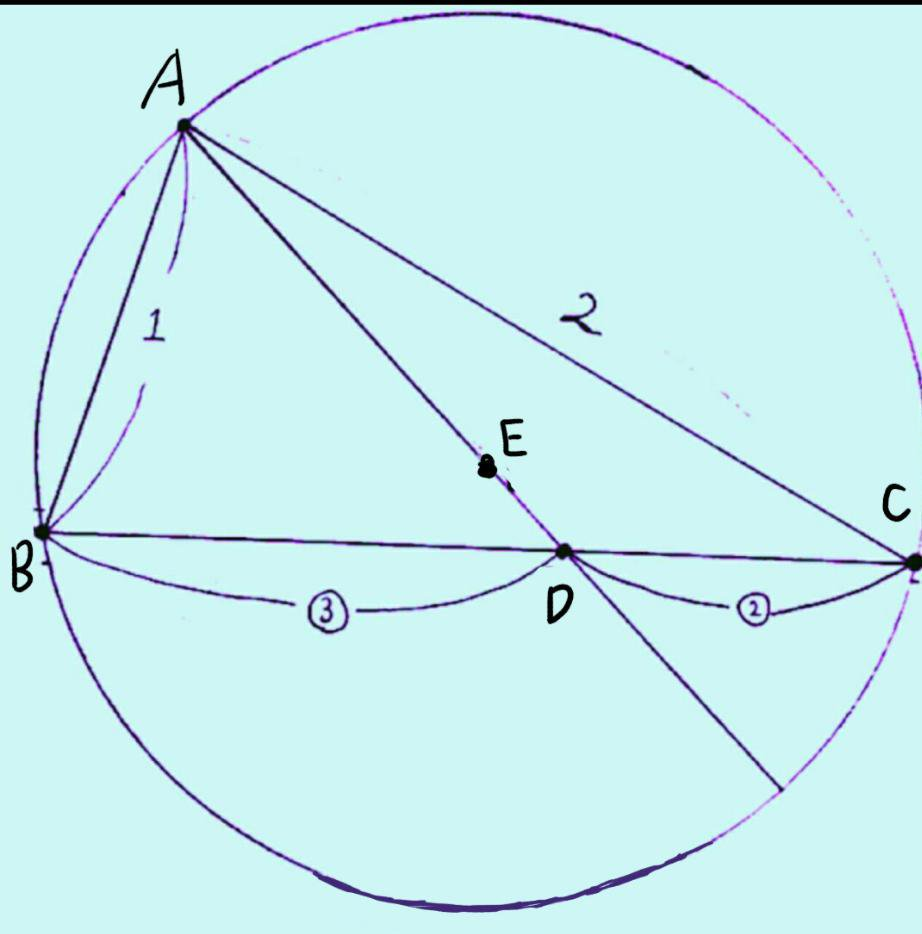
\includegraphics[bb=0 0 922 934,width=0.7\linewidth]{../problems/Q_070/Q_070.jpg}
 \end{figure}
\end{thm}

ここに解答を記述する。
